%
% ------------------------------------------------------------------------------
	\index{PSHA!Input model}
%
In this Chapter we discuss the two main information blocks OpenQuake 
requires to perform a calculation: (1) a PSHA input model and (2) 
Calculation Settings.

A \gls{pshainputmodel} defines the properties of the seismic sources 
of engineering  interest within the region considered in the analysis and the 
models capable to describe - once a rupture occurred in a given position - the 
properties of the shaking expected at the site. 
%
A PSHA input model contains two main objects: the \emph{Seismic Sources System} 
and the \emph{Ground Motion System}. 
%
The former specifies location, geometry, and seismicity properties of seismic 
sources and potential epistemic uncertainties affecting this information. 
%
The latter describes the details of the ground motion prediction equations to 
be adopted in the calculation and the related epistemic uncertainties. 
%
Therefore, the PSHA input models for OpenQuake are always defined using two 
logic tree structures, one describing epistemic uncertainties associated 
with the creation of the ERF - called \emph{Seismic Sources logic tree} - 
	\index{Logic Tree!Seismic Sources}
the other - called \emph{Ground Motion logic tree} - takes into account 
the uncertainties connected with the use of models capable to predict the 
expected ground motion at the site. 
	\index{Logic Tree!Ground Motion}
%
In cases where the epistemic uncertainties are not considered, the logic tree 
structure simply consists of one branching level with just one branch (with 
weight equal to 1).

Calculation settings specifies for example the typology of results required,
the site or the sites where to compute the hazard and, the calculation
methodology to apply.

The organisation of this chapter is the following.  
Section \ref{hazard:seismic_source_types} contains a description of the 
seismicsource type currently supported by OpenQuake. 
The logic tree structure supported in OQ is described in Section 
\ref{hazard:logic_tree} while the PSHA input model is discussed in 
Section \ref{hazard:pshainputmodel}.
Finally, Section \ref{hazard:calculation_settings} provides an outlook 
of the hazard specific calculation setting supported by OpenQuake.
%
% ------------------------------------------------------------------------------
\section[OpenQuake seismic source typologies]{OpenQuake seismic source 
typologies}
\label{hazard:seismic_source_types}
\input{./Part_Hazard/unifiedmodel/seismicSourceTypes.tex}
%
% ------------------------------------------------------------------------------
\section{Logic-tree description}
\label{hazard:logic_tree}
%
% ------------------------------------------------------------------------------
\section{Logic-tree description}
\label{hazard:logic_tree}
Logic-trees are a tool designed to consider in a systematic manner the 
epistemic uncertainties of models and parameters included in a hazard 
analysis.
% ..............................................................................
% . . . . . . . . . . . . . . . . . . . . . . . . . . . . . . . . . . . > Figure
\renewcommand{\psedge}{\ncdiag[armA=0,angleB=180,armB=1cm]}
\begin{figure}[!hb]
\input{./Part_Hazard/pstricks/sslt_absolute.tex}
\caption{An example of branch set used to account for the epistemic 
uncertainties on faults dip angle; in this case each branch contains a value 
of the dip.}
\label{fig:logic_tree_branching_levels}
\end{figure}
% . . . . . . . . . . . . . . . . . . . . . . . . . . . . . . . . . . . < Figure
% ..............................................................................

A logic tree cont\-ains three main elements:
\begin{itemize}
\item Branching Level
\item Branch Set
\item Branch
\end{itemize}
%
A \emph{branching level}, expresses the distance of a given element from the 
root of the logic tree; in the simplest case each branching level corresponds 
to a single type uncertainty (e.g. maximum magnitude). 
Indicatively, we can say that the larger the number of branching levels in a 
logic structure the larger is its complexity.
%
\index{Logic Tree!Branch set}
A \emph{branch set} describes an uncertainty model; for example - as previously 
mentioned - a model accounting for the epistemic uncertainties connected with 
the definition of maximum magnitude. A branch set contains of a number of 
mutually exclusive and collectively exhaustive options \citep{bommer2008}. 
%
Finally, a \emph{branch} represent a particular alternative in a branch set and 
therefore it refers to an uncertainty model and has a weight expressing - 
according to different interpretations available in the literature 
- ``probabilities or simply subjective indications of relative merit'' 
\citep[][page 999]{bommer2008}.
	\index{Logic Tree!Branch}

%
In more detail, a branch set - the fundamental component in our logic tree data 
model - consists on (1) the parameter (or model) affected 
by uncertainty, (2) the specification of the type of uncertainty (3) the 
listing of the - mutually exclusive and collectively exhaustive 
- alternative hypotheses (4) a weight for each hypothesis, 
(5) a flag specifying if the branches are (totally) correlated and, (6) the 
index of the branches of the previous level - or the subset of seismic 
sources - to which this branch set applies.

Figure \ref{fig:logic_tree_branching_levels} depicts a branch 
set fixing epistemic uncertainties on the dip angle of simple 
fault sources. In this case the possible values of the dip are specified
on each branch composing the branch set (i.e. 30, 45 and 60 degrees). This 
means that these three values are the only ones admitted for all the sources 
included in the initial seismic source model considered. 
%
Figure \ref{fig:logic_tree_branching_levels_1} also shows a branch
set defining epistemic uncertainties on the dip angle 
of simple fault sources. In this case, however, the values specified for each 
branch aren't absolute dip angles but instead differential values to be added - 
or subtracted - to the dip value specified for each simple fault source 
contained in the initial seismic sources model.

% ..............................................................................
% . . . . . . . . . . . . . . . . . . . . . . . . . . . . . . . . . . . > Figure
\renewcommand{\psedge}{\ncdiag[armA=0,angleB=180,armB=1cm]}
\begin{figure}
%\fbox{\begin{minipage}{\textwidth}
\hfill \\
\textcolor{blue01}{\emph{Branch set definition}}: \dotfill
	Simple Fault Dip Angle \\
\textcolor{blue01}{\emph{Branch set uncertainty type}}: \dotfill
	Relative values \\
\textcolor{blue01}{\emph{Applies to}}: \dotfill
	All previous branches \\
\textcolor{blue01}{\emph{Correlated branches}}: \dotfill Yes \\
\hfill \\
	\centering
	\begin{psTree}[treemode=R,levelsep=*2cm]
			{\Tr{ }}
		\begin{psTree}[treemode=R]{
			\Tr{\parbox[b]{4cm}{ value = -15$^\circ$ 
				\newline weight=w$_1$}}}%
		\end{psTree}%
		\begin{psTree}[treemode=R,treenodesize=1cm]{
			\Tr{\parbox[b]{4cm}{ value = 0$^\circ$ 
				\newline weight=w$_2$}}}%
		\end{psTree}%
		\begin{psTree}[treemode=R]{
			\Tr{\parbox[b]{4cm}{ value = +15$^\circ$ 
				\newline weight=w$_3$}}}%
		\end{psTree}%
	\end{psTree}%
\\ \hfill \\
%\end{minipage}} % End of fbox
\caption{An example of branch set used to account for the epistemic 
uncertainties on faults dip angle; in this case each branch contains a 
differential from a default dip value indicated for each source in the 
initial seismic sources model.}
\label{fig:logic_tree_branching_levels_1}
\end{figure}
% . . . . . . . . . . . . . . . . . . . . . . . . . . . . . . . . . . . < Figure
% ..............................................................................
Two or more branch sets they can be combined in flexible fashion (i.e. 
concatenated) to create an entire logic-tree structure.
Figure \ref{fig:logic_tree_schema} shows an example of a logic tree 
created by combining the two branch sets described in the upper part of the
figure. 
The first branch set accounts for epistemic uncertainties connected with 
the dip of simple fault sources whilst the second specifies 
the epistemic uncertainties relative to the depth to the top of rupture  
(this branching level also applies to simple faults included in the model).
% ..............................................................................
% . . . . . . . . . . . . . . . . . . . . . . . . . . . . . . . . . . . > Figure
\begin{figure}[!h]
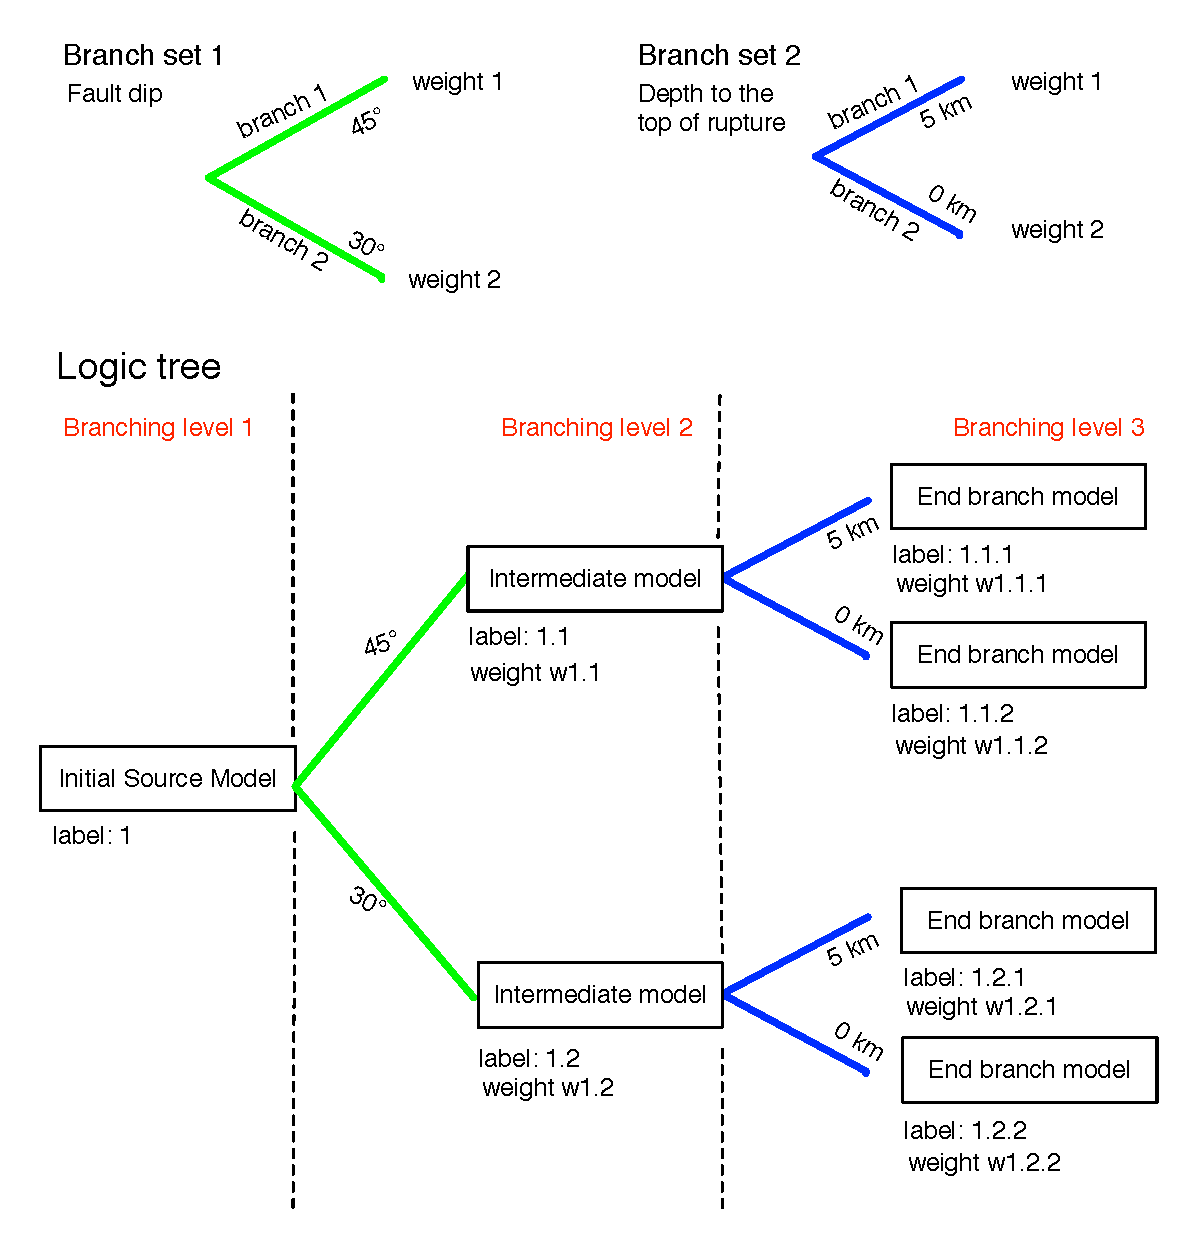
\includegraphics[width=15cm]{./Figures/Part_Hazard/logic_tree_schema.eps}
\caption{Example of a logic tree structure as defined in OpenQuake. The upper
part of the Figure depicts two branch sets.}
\label{fig:logic_tree_schema}
\end{figure}
% . . . . . . . . . . . . . . . . . . . . . . . . . . . . . . . . . . . < Figure
% ..............................................................................
%

This data model permits a very general definitions of logic tree 
structures. For instance, a non-symmetric logic tree can be easily 
created by placing multiple branch sets in the same branching level, each 
branch set being connected to a specific branch of a branch set defined in a
previous branching level. Figure \ref{fig:LogicTreeGeneralStructure}) shows a 
general example of a logic tree structure supported by OpenQuake logic tree 
data model. 

% ..............................................................................
% . . . . . . . . . . . . . . . . . . . . . . . . . . . . . . . . . . . > Figure
\begin{figure}
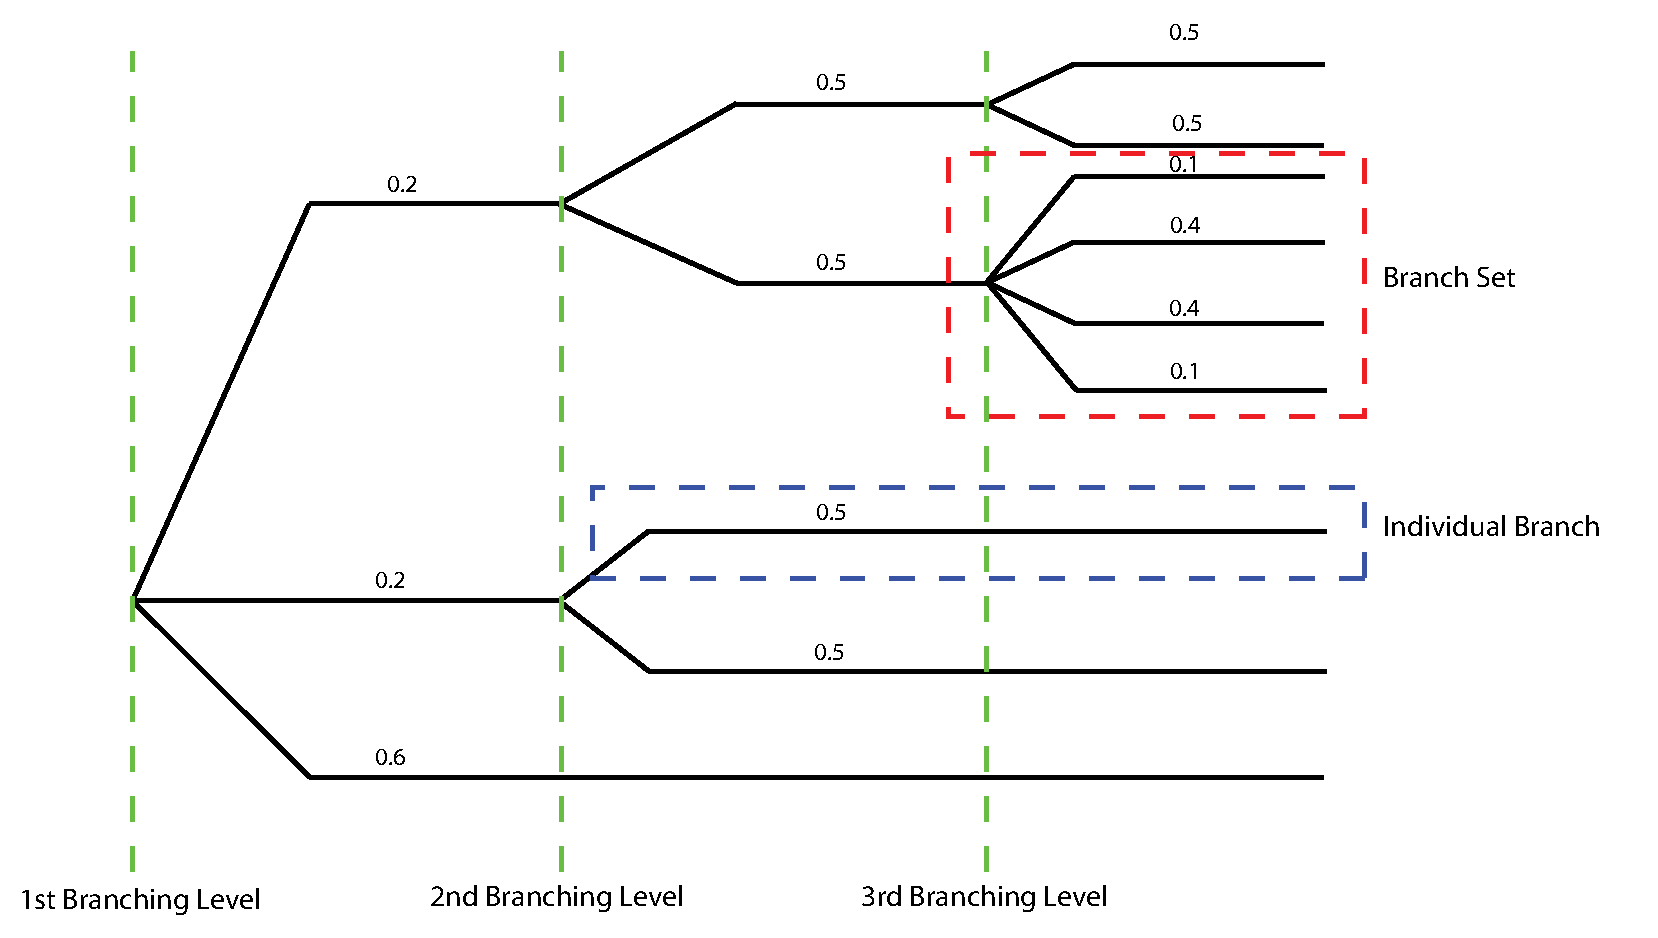
\includegraphics[width=15cm]{./Figures/Part_Hazard/LogicTreeGeneralStructure.eps}
\caption{Logic Tree data structure as defined in terms of individual branches, 
branch sets, and branching levels.}
\label{fig:LogicTreeGeneralStructure}
\end{figure}
% . . . . . . . . . . . . . . . . . . . . . . . . . . . . . . . . . . . < Figure
% ..............................................................................

We use this logic tree description to specify the structure of the Seismic 
Sources Logic Tree as well as for the Ground Motion Models Logic Tree. 
%  - - - - - - - - - - - - - - - - - - - - - - - - - - - - - - - - - - - - - - -
\subsection{Source Model Logic Tree}
\label{hazard:source_model_logic_tree}
%
In the current version of OpenQuake, a seismic sources model logic tree can be 
defined according to the following schema:
\begin{itemize}
\item The first branching level is assumed describing one or more "alternative" 
initial seismic source models.
\item Subsequent branching levels define source parameters uncertainties. 
Parameters uncertainties are applied independently to each seismic source 
in a source model. That is epistemic uncertainties are assumed uncorrelated 
between different seismic sources.
\item One branch set can be defined for branching level, thus assuming 
symmetric logic tree definition only.
\end{itemize}
%
The possibility of defining multiple source models in the first branching 
level responds to the need of modern PSHA of considering alternative source 
models (as derived by different expert opinions, for instance). 
%
Subsequent branching levels define the epistemic uncertainties that 
apply to parameters characterizing seismic sources. The  
epistemic uncertainties related to these parameters are implemented as 
\emph{rules}, that is as algorithms describing how this parameter has to be 
modified. 
%
The major advantage of using a rule-based approach is that a user does not 
need to a provide an input file containing a source model definition 
corresponding to a specific epistemic uncertainty, that is instead computed 
and applied on the fly to the initial model.
%
% ..............................................................................
% . . . . . . . . . . . . . . . . . . . . . . . . . . . . . . . . . . . > Figure
\begin{figure}
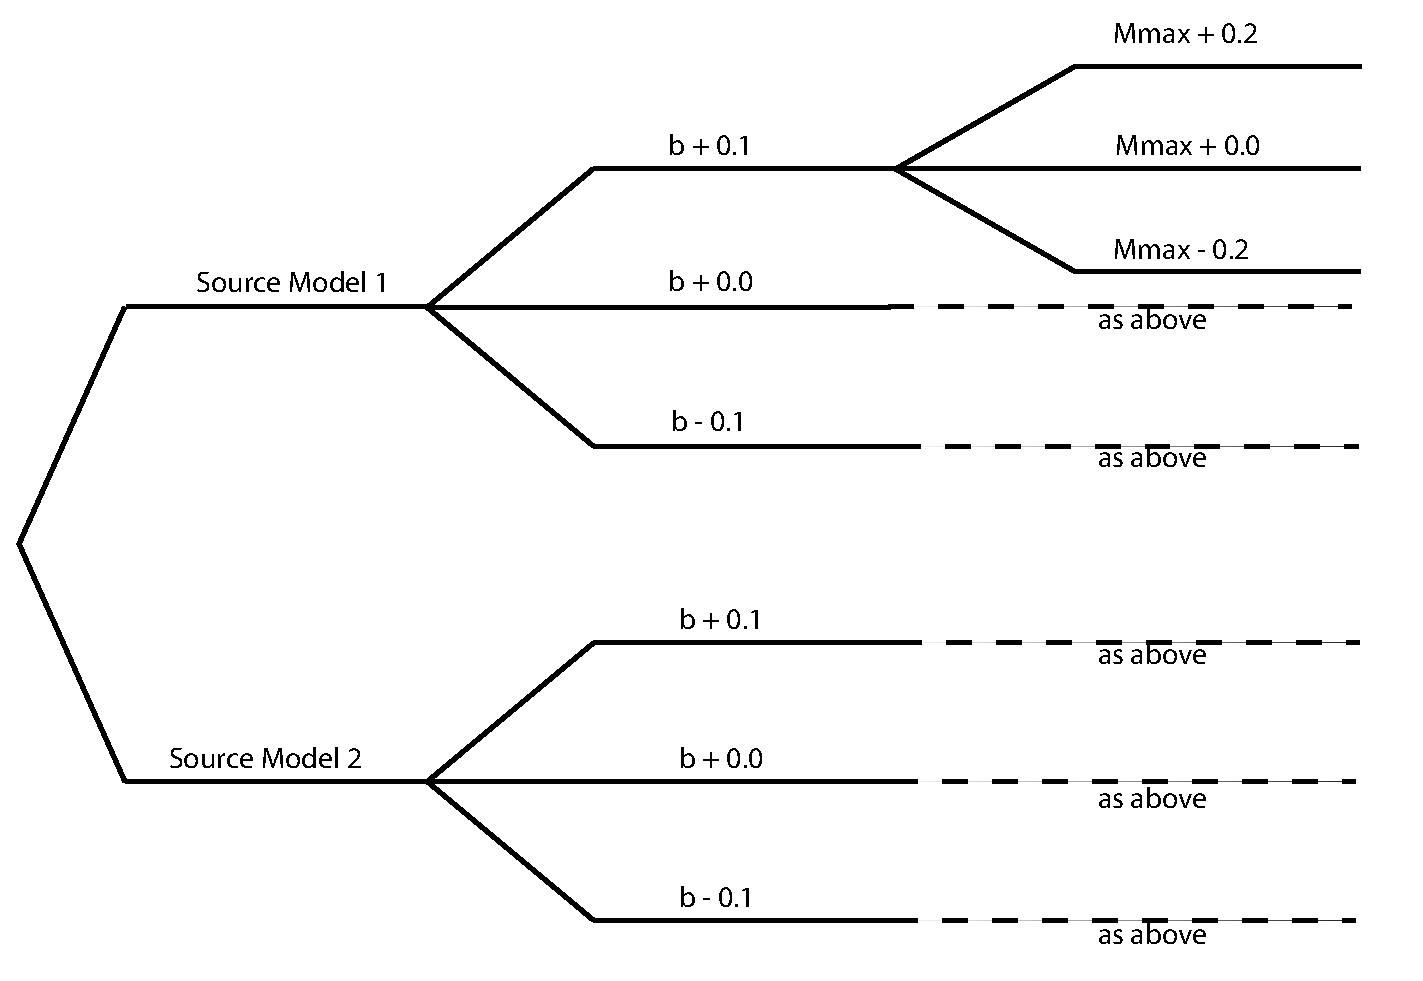
\includegraphics[width=15cm]{./Figures/Part_Hazard/SourceModelLogicTree.eps}
\caption{Example of Seismic Sources Logic Tree. The first branching level defines
two alternative source models (Source Model 1, Source Model 2). The second 
branching level defines uncertainties in b value (increment of 0.1, 0.0, -0.1).
The third branching level defines uncertainties in maximum magnitude 
(increments of 0.2, 0.0, -0.2).}
\label{fig:SourceModelLogicTree}
\end{figure}
% . . . . . . . . . . . . . . . . . . . . . . . . . . . . . . . . . . . < Figure
% ..............................................................................
%

The current version of OpenQuake offers two built-in rules:
\begin{itemize}
\item Gutenberg-Richter b value uncertainties. The user can specify a set 
of increments (positive or negative) that are added to Gutenberg-Richter 
b values. Conservation of total moment rate is assumed.
\item Gutenberg-Richter maximum magnitude uncertainties. The user can specify
a set of increments (positive or negative) that are added to Gutenberg-Richter 
maximum magnitude values. Conservation of total moment rate is assumed.
\end{itemize}
Figure \ref{fig:SourceModelLogicTree} depicts a source model logic tree that 
can be defined with the options currently present in OpenQuake.

The above mentioned rules are only a sample of possible source model epistemic 
uncertainties, and future versions of OpenQuake will provide a broader spectrum
of built-in epistemic uncertainties. Currently, rules are applied to all 
sources. Option to apply rules only to specific sources will be also supported 
in the future.
%  - - - - - - - - - - - - - - - - - - - - - - - - - - - - - - - - - - - - - - -
\subsection{GMPE Logic Tree}
\label{hazard:gmpe_logic_tree}
The GMPE Logic Tree allows a user to consider multiple ground motion prediction
equations in the hazard modeling. Given that GMPEs are often, or can be, 
associated to specific tectonic region types, OpenQuake allows the definition 
of multiple GMPE logic trees, one for each tectonic region type considered in 
the source model. In the current version, a GMPE logic tree can have only one 
branching level, containing only one branch set, where each individual branch 
is associated to a specific GMPE. With the current setting, epistemic 
uncertainties coming from different models can be taken into account, but 
epistemic uncertainties inside each model cannot be captured.
Figure \ref{fig:GMPELogicTree} schematically shows GMPE logic trees that can 
be currently defined in OpenQuake.
% ..............................................................................
% . . . . . . . . . . . . . . . . . . . . . . . . . . . . . . . . . . . > Figure 
\renewcommand{\psedge}{\ncdiag[armA=0,angleB=180,armB=1cm]}
\begin{figure}
\input{./Part_Hazard/pstricks/logicTreeGmpes.tex}
\caption{Examples of GMPE Logic Trees. One for active shallow crust (considering
three GMPEs) and one for subduction interface (considering two GMPEs).}
\label{fig:GMPELogicTree}
\end{figure}

% . . . . . . . . . . . . . . . . . . . . . . . . . . . . . . . . . . . < Figure
% ..............................................................................
%
% ------------------------------------------------------------------------------
\section{The PSHA input model}
\label{hazard:pshainputmodel}
\index{PSHA!Input model}
The PSHA Input Model is the container of the information necessary to specify 
(1) position, shape, activity rates and associated epistemic uncertainties
of the seismic sources of engineering importance within a defined area and (2) 
the ground motion models and the associated uncertainties to be used for PSHA
calculation.
% 
The two corresponding objects included in the PSHA Input Model are the 
Seismic Sources System and the Ground Motion System.
% ..............................................................................
% . . . . . . . . . . . . . . . . . . . . . . . . . . . . . . . . . . . > Figure
%\begin{figure}
%\centering
%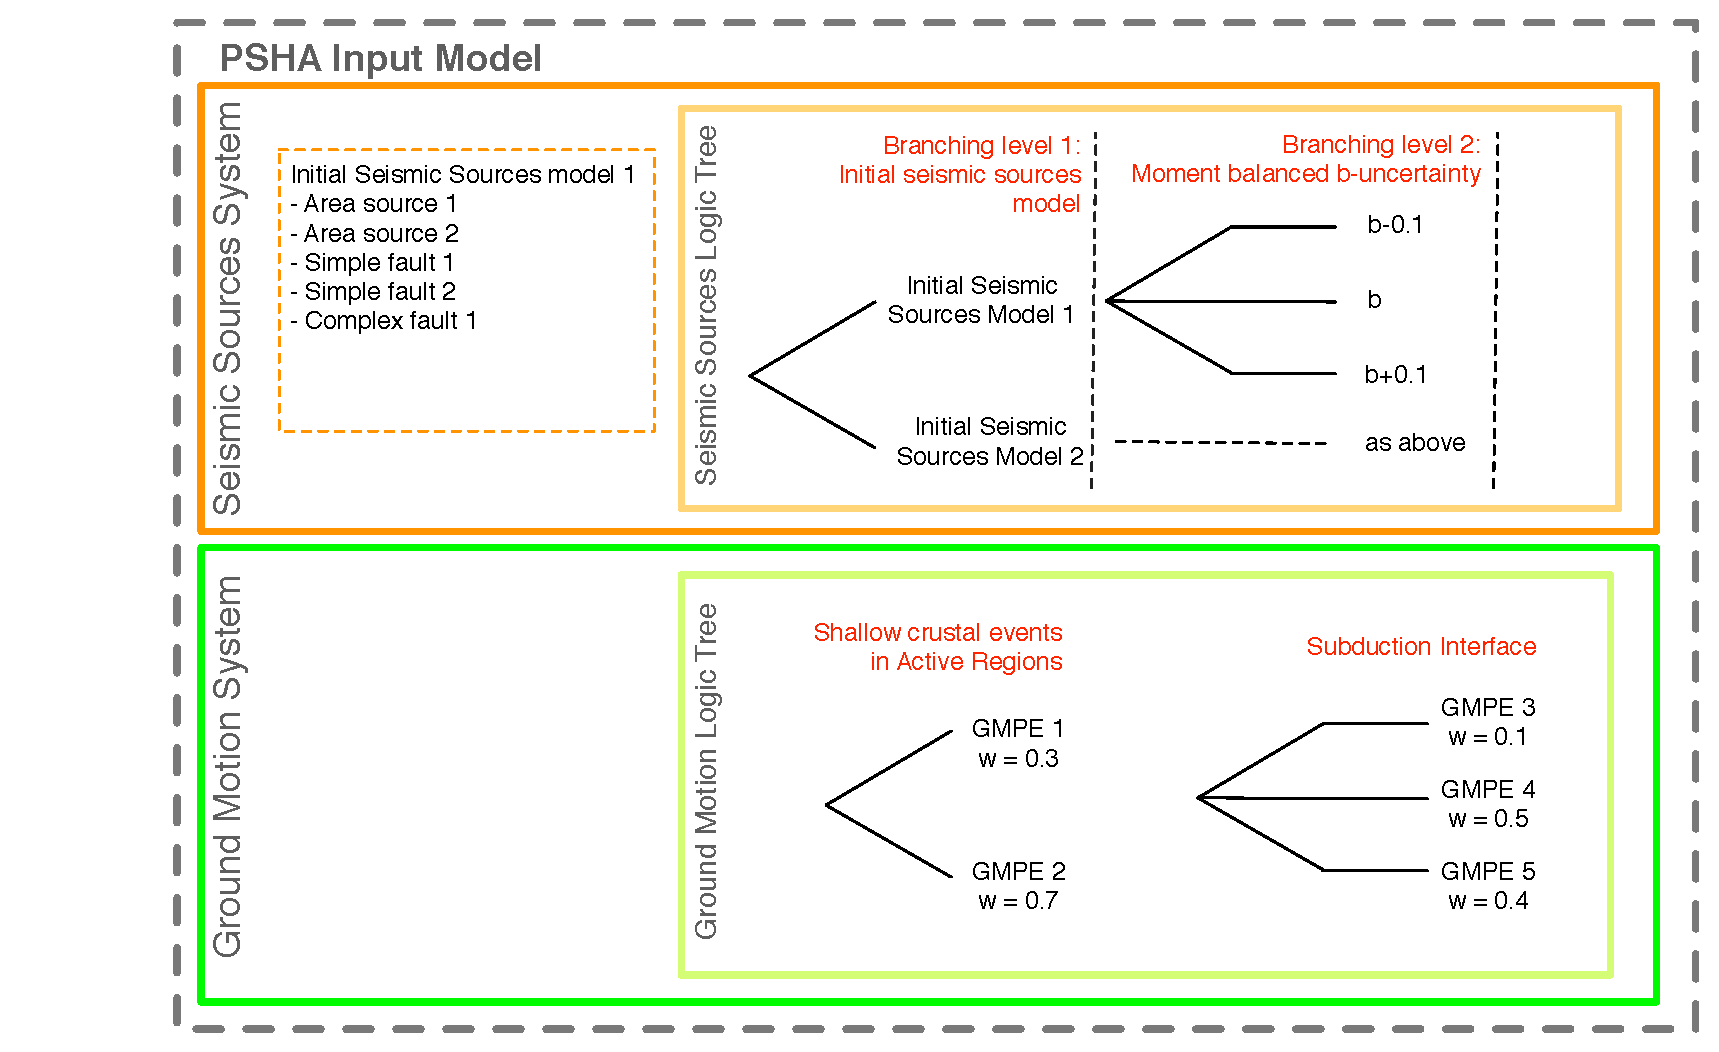
\includegraphics[width=15cm]{./Figures/Part_Hazard/psha_input_model.eps}
%\caption{Schema describing the main elements composing the PSHA Input Model. 
%The orange box represents the Seismic Sources System while the green box 
%portray the ground motion system.}
%\label{fig:psha_input_model}
%\end{figure}
% . . . . . . . . . . . . . . . . . . . . . . . . . . . . . . . . . . . < Figure
% ..............................................................................
%  - - - - - - - - - - - - - - - - - - - - - - - - - - - - - - - - - - - - - - -
\subsection{The Seismic Sources System}
\index{Seismic Sources!System}
The \gls{seismicsourcesystem} is the ensemble of one or several 
\glspl{initialseismicsourcemodel} and the \gls{seismicsourcelogictree}.
%
The initial seismic source model is a list of \gls{seismicsourcedata}
(the typologies of sources admitted is described in Section
\ref{hazard:seismic_source_types}).
%
Usually, a seismic source model contains one or several seismic 
sources accounting for distributed seismicity (e.g. area sources, 
grid sources) and - eventually - one or several individual seismic 
sources.

The \gls{seismicsourcelogictree} describes the epistemic uncertainties 
associated with the parameters used to characterize the Initial 
Seismic Sources models. 
% 
Though this logic tree the user can take into account the epistemic
uncertainties associated with almost all the parameters characterizing
each source typology. 
% 
Currently OpenQuake contains just a limited number of logic tree
branch set types. 

%  - - - - - - - - - - - - - - - - - - - - - - - - - - - - - - - - - - - - - - -
\subsubsection{Seismic Sources Logic Tree}
\label{hazard:source_model_logic_tree}
\index{Logic Tree!Seismic Sources}
%
In the current version of OpenQuake, a \gls{seismicsourcelogictree} can be 
defined according to the following schema:
\begin{itemize}
\item The first branching level is assumed describing one or more "alternative" 
initial seismic source models.
\item Subsequent branching levels define source parameters uncertainties. 
Parameters uncertainties are applied independently to each seismic source 
in a source model. That is epistemic uncertainties are assumed uncorrelated 
between different seismic sources.
\item One branch set can be defined for branching level, thus assuming 
symmetric logic tree definition only.
\end{itemize}
%
The possibility of defining multiple source models in the first branching 
level responds to the need of modern PSHA of considering alternative source 
models (as derived by different expert opinions, for instance). 
%
Subsequent branching levels define the epistemic uncertainties that 
apply to parameters characterizing seismic sources. The  
epistemic uncertainties related to these parameters are implemented as 
\emph{rules}, that is as algorithms describing how this parameter has to be 
modified. 
%
The major advantage of using a rule-based approach is that a user does not 
need to a provide an input file containing a source model definition 
corresponding to a specific epistemic uncertainty, that is instead computed 
and applied on the fly to the initial model.
%
% ..............................................................................
% . . . . . . . . . . . . . . . . . . . . . . . . . . . . . . . . . . . > Figure
\begin{figure}
%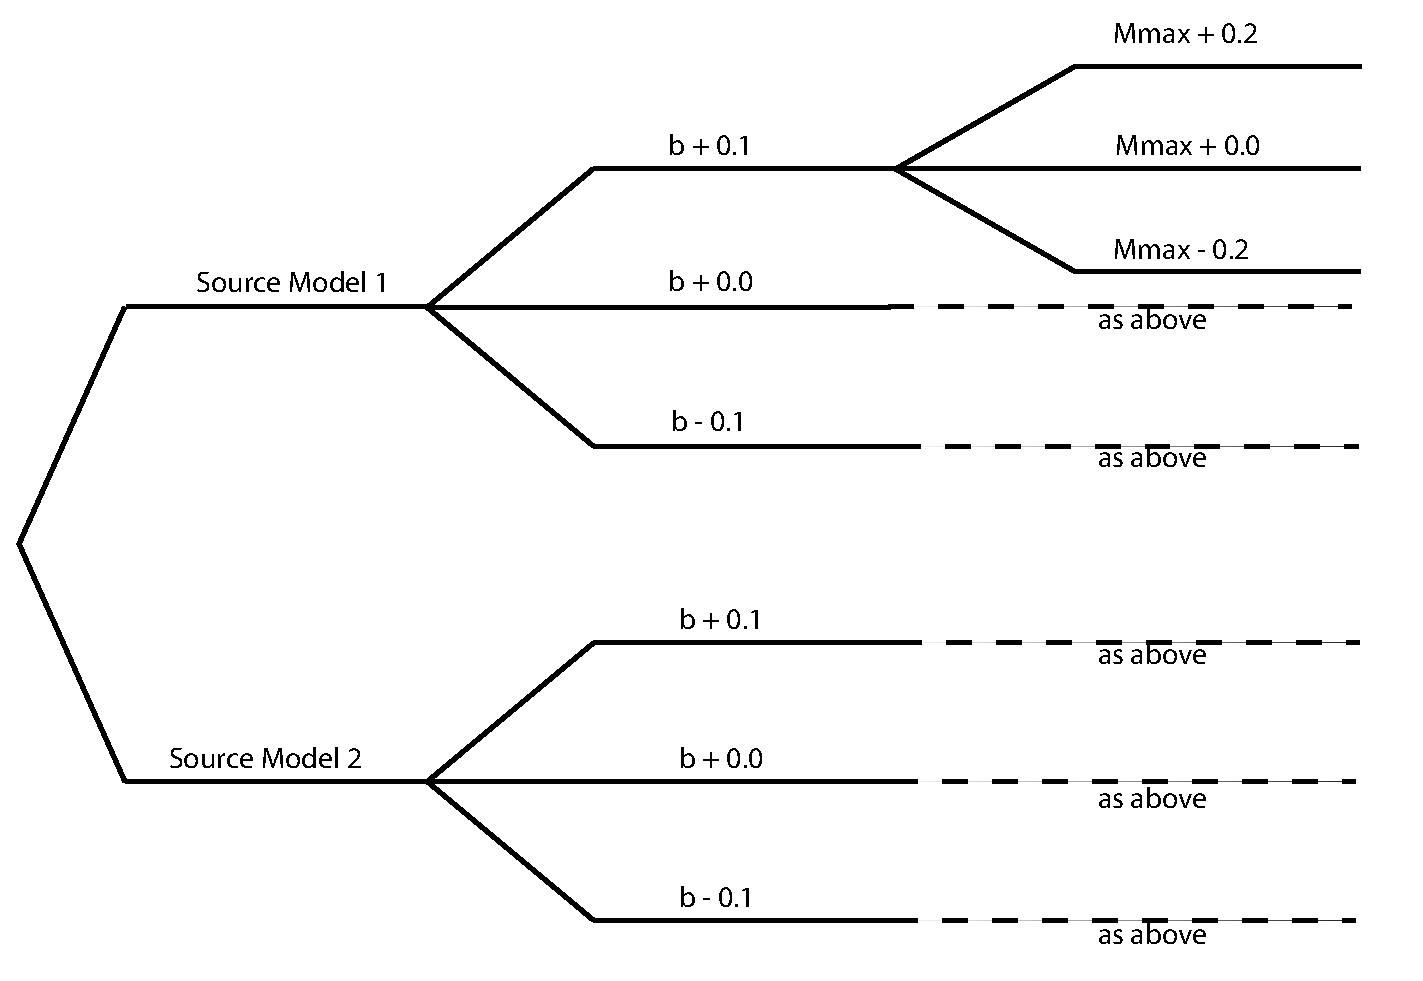
\includegraphics[width=15cm]{./Figures/Part_Hazard/SourceModelLogicTree.eps}
\pstree[treemode=R,levelsep=20ex]{\Tr{}}{
    \pstree{\Tr{\parbox[b]{2cm}{Initial Seismic Sources model 1}}}{
            \pstree{\Tr{  \parbox[b]{1cm}{b-0.1}  }}{
            	\Tr{ \parbox[b]{2cm}{mmax-0.2} }
            	\Tr{ \parbox[b]{2cm}{mmax} }
            	\Tr{ \parbox[b]{2cm}{mmax+0.2} }
    		}
            \pstree{\Tr{ \parbox[b]{1cm}{b} }}{
            	\Tr{ \parbox[b]{2cm}{as above} }
    		}
            \pstree{\Tr{ \parbox[b]{1cm}{b+0.1} }}{
            	\Tr{ \parbox[b]{2cm}{as above} }
    		}
    }
    \pstree{\Tr{\parbox[b]{2cm}{Initial Seismic Sources model 2}}}{
            \pstree{\Tr{ \parbox[b]{1cm}{b-0.1} }}{
            	\Tr{ \parbox[b]{2cm}{as above} }
    		}
            \pstree{\Tr{ \parbox[b]{1cm}{b}}}{
            	\Tr{ \parbox[b]{2cm}{as above} }
    		}
            \pstree{\Tr{ \parbox[b]{1cm}{b+0.1} }}{
            	\Tr{ \parbox[b]{2cm}{as above} }
    		}
    }                 
}
\hfill \\
\caption{Example of Seismic Sources Logic Tree. The first branching level defines
two alternative source models (Source Model 1, Source Model 2). The second 
branching level defines uncertainties in b value (increment of 0.1, 0.0, -0.1).
The third branching level defines uncertainties in maximum magnitude 
(increments of 0.2, 0.0, -0.2).}
\label{fig:SourceModelLogicTree}
\end{figure}
% . . . . . . . . . . . . . . . . . . . . . . . . . . . . . . . . . . . < Figure
% ..............................................................................
%
% . . . . . . . . . . . . . . . . . . . . . . . . . . . . . . . . . . . . . . .
\subsubsection{Supported branch set typologies}
The current version of OpenQuake offers only two built-in typologies of 
branch set. They are only a sample of the possible seismic source model 
epistemic uncertainties, and future versions of OpenQuake will provide 
a broader spectrum of built-in branch sets accounting for distinct 
types of epistemic uncertainties. 

Figure \ref{fig:SourceModelLogicTree} depicts a source model logic tree that 
can be defined with the options currently present in OpenQuake.
%
\paragraph{Gutenberg-Richter b value uncertainties}
This is the \gls{branchset} in the second \gls{branchinglevel} of the 
seismic source logic tree depicted in Figure \ref{fig:SourceModelLogicTree}. 
This \gls{branchset}, contains a number of branches. Each one has associated: 
(1) a differential value to be added or subtracted to the Gutenberg-Richter b 
value of each source as specified in the \gls{initialseismicsourcemodel} and 
(2) a weight.
Within this \gls{branchset} conservation of total moment rate 
(corresponding to the one specified in the initial seismic source model) 
is assumed.
%
\paragraph{Gutenberg-Richter maximum magnitude uncertainties}
For this \gls{branchset} the user can specify for each \gls{branch} a 
value (positive or negative) to be added to the Gutenberg-Richter maximum 
magnitude values. 
%
Within this \gls{branchset} conservation of total moment rate 
(corresponding to the one specified in the initial seismic source model) 
is assumed.
%  - - - - - - - - - - - - - - - - - - - - - - - - - - - - - - - - - - - - - - -
\subsection{The Ground Motion System}
\index{Ground Motion!System}
% Table: list of GMPEs currently supported by OQ
\input{./Part_Hazard/tables/gmpeslist.tex}
%
The Ground Motion System is a combination of one or several logic 
trees each one associated with a specific tectonic region or group 
of sources (this second option is still not supported in OQ).
%
Each Ground Motion Logic Tree specifies the alternative Ground Motion 
models available for a particular group of sources (e.g. subduction 
interface sources).

OpenQuake provides only hardcoded \gls{acr:gmpe} 
and misses of a mechanisms allowing the user to specify new GMPEs. 
This is a feature that we may think to introduce in the future. 

Table \ref{tab:OQ_GMPEs} provides a list of the Ground Motion Prediction 
Equations supported. 

The vast majority are GMPEs implemented in OpenSHA with just a couple 
of developed in the course of the GEM1 project. New GMPEs are expected 
to be added soon with the contribution of some GEM's Regional Programmes.

%  - - - - - - - - - - - - - - - - - - - - - - - - - - - - - - - - - - - - - - -
\subsubsection{Ground Motion Logic Tree}
\label{hazard:gmpe_logic_tree}
\index{Logic Tree!Ground Motion}
The Ground Motion Logic Tree accounts for epistemic uncertainties related 
to the Ground Motion models.  
%
Given that ground motion models are often, or can be, associated to 
specific tectonic region,  OpenQuake supports the definition of multiple 
GMPE logic trees, one for each tectonic region type considered in 
the source model. 
% 
For example, if a PSHA Input model contains seismic sources belonging to 


In the current version, a GMPE logic tree can have only one 
branching level, containing only one branch set, where each individual branch 
is associated to a specific GMPE. With the current setting, epistemic 
uncertainties coming from different models can be taken into account, but 
epistemic uncertainties inside each model cannot be captured.
Figure \ref{fig:GMPELogicTree} schematically shows GMPE logic trees that can 
be currently defined in OpenQuake.
% ..............................................................................
% . . . . . . . . . . . . . . . . . . . . . . . . . . . . . . . . . . . > Figure 
\renewcommand{\psedge}{\ncdiag[armA=0,angleB=180,armB=1cm]}
\begin{figure}[!hb]
\centering
\input{./Part_Hazard/pstricks/logicTreeGmpes.tex}
\caption{Examples of Ground Motion Logic Trees. The first specifies ground
motion models for active shallow crust (in this case we consider three GMPEs) 
the second defines the ground motion models to adopt for subduction interface 
sources (in the example depicted above we consider two GMPEs).}
\label{fig:GMPELogicTree}
\end{figure}

% . . . . . . . . . . . . . . . . . . . . . . . . . . . . . . . . . . . < Figure
% ..............................................................................

%
% ------------------------------------------------------------------------------
\section{Calculation settings}
\label{hazard:calculation_settings}
\input{./Part_Hazard/unifiedmodel/calculationsettings.tex}






